\documentclass[11pt,a4paper]{article}

\usepackage[utf8]{inputenc}
\usepackage[T1]{fontenc}
\usepackage{lmodern}
\usepackage[margin=2.2cm,top=2.2cm,bottom=2.2cm]{geometry}
\usepackage{graphicx}
\usepackage{amsmath,amssymb}
\usepackage{booktabs}
\usepackage{hyperref}
\usepackage{caption}
\usepackage{fancyhdr}
\usepackage{float}
\usepackage{parskip}

\renewcommand{\tablename}{Tabla}
\renewcommand{\figurename}{Figura}

\hypersetup{
    colorlinks=true,
    linkcolor=black,
    urlcolor=blue
}

\pagestyle{fancy}
\fancyhf{}
\fancyhead[L]{\small Visión Artificial y Lenguaje Natural (2026)}
\fancyhead[R]{\small Trabajo Práctico Integrador -- Retinografía}
\fancyfoot[C]{\thepage}

\begin{document}

% ==========================================
% 1. CARÁTULA Y DATOS INSTITUCIONALES
% ==========================================
\thispagestyle{empty}
\begin{center}
    \vspace*{1.0cm}
    {\Large \textbf{Licenciatura en Inteligencia Artificial}}\\[0.3cm]
    {\large \textbf{Materia:} 2026-1IA1(1) Visión Artificial y Lenguaje Natural}\\[1.5cm]
    
    \rule{\linewidth}{0.5mm} \\[0.4cm]
    {\LARGE \textbf{Trabajo Práctico Integrador: Visión Artificial}}\\[0.3cm]
    {\Large Pipeline de Procesamiento y Metrología en Retinografía Vascular Digital}\\[0.2cm]
    \rule{\linewidth}{0.5mm} \\[1.5cm]

    \begin{minipage}{0.85\textwidth}
        \textbf{Caso Seleccionado:} Img 3 -- Retinografía Vascular Digital (Recurso: \texttt{Retina / 3.png})\\[0.4cm]
        \textbf{Herramienta Utilizada:} ImageJ.js (Versión Online en el navegador / No-Code GUI)\\[0.6cm]
        \textbf{Profesores:}
        \begin{itemize}
            \item Martín Gustavo Casatti
            \item Sebastián Federico Oliva
        \end{itemize}
        \vspace{0.3cm}
        \textbf{Integrantes del Grupo:}
        \begin{itemize}
            \item \textbf{Bringas, Mateo Lautaro} -- Legajo: 435719
            \item \textbf{Castro, Cristian Leonel} -- Legajo: 435837
            \item \textbf{Garcia Pintos, Valentín} -- Legajo: 435804
        \end{itemize}
    \end{minipage}

    \vfill
    {\large Ciclo Lectivo 2026}
\end{center}

\newpage
\setcounter{page}{2}

% ==========================================
% 2. DIAGNÓSTICO FOTOMÉTRICO Y DE ADQUISICIÓN
% ==========================================
\section{Diagnóstico Fotométrico y de Adquisición}

Para comenzar el trabajo en Fiji/ImageJ, abrimos la imagen \texttt{3.png} ($1024 \times 680$ píxeles). Al tratarse de una imagen a color (RGB) de fondo de ojo, el primer paso antes de pasar a 8 bits fue evaluar los canales por separado mediante \texttt{Image > Color > Split Channels}. 

Observamos que el canal Rojo está muy saturado (los vasos casi no se distinguen del tejido) y el canal Azul es demasiado oscuro y ruidoso. En cambio, el \textbf{Canal Verde (G)} muestra el mejor contraste porque la sangre absorbe mucha luz en esa longitud de onda, haciendo que las venas y arterias se vean bien oscuras respecto al fondo de la retina. Por eso nos quedamos con el canal verde como imagen monocromática de 8 bits (valores discretos en $[0, 255]$).

\begin{figure}[H]
    \centering
    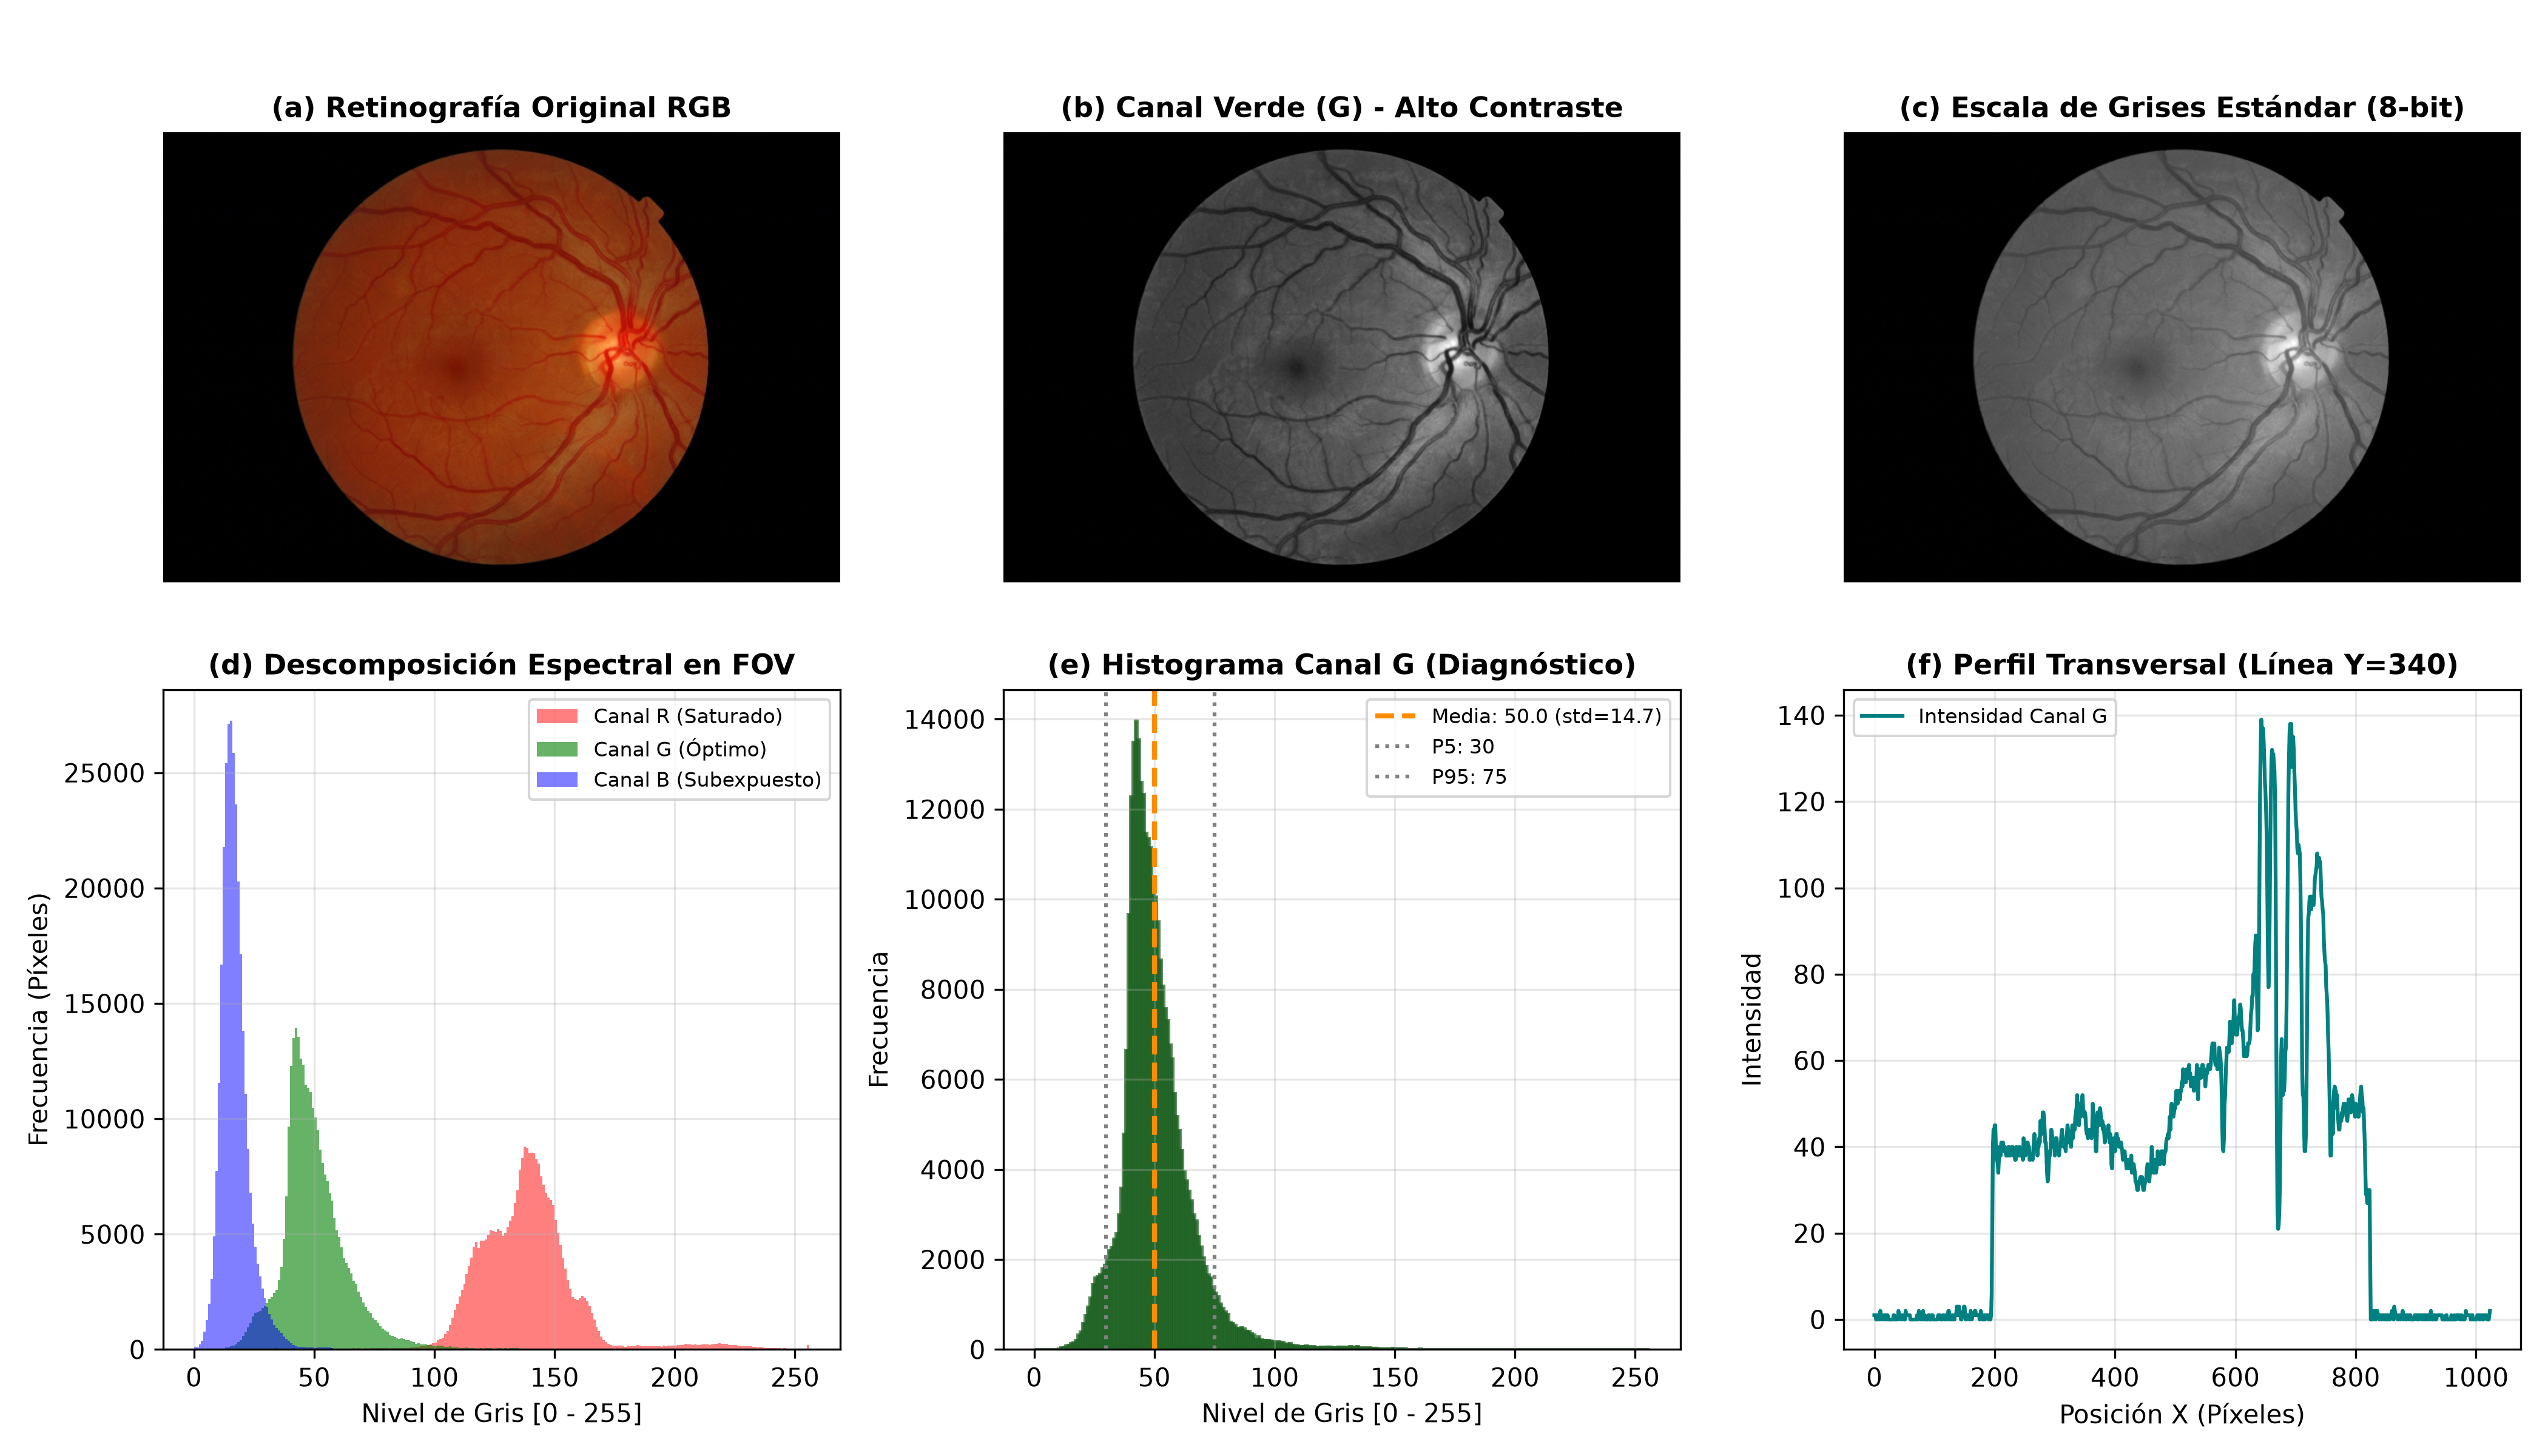
\includegraphics[width=0.92\textwidth]{figuras/fig1_diagnostico_histograma.png}
    \caption{Separación de canales, imagen en 8 bits y análisis del histograma de niveles de gris sobre la retina.}
    \label{fig:diagnostico}
\end{figure}

\textbf{Interpretación del Histograma y Rango Dinámico:}
\begin{itemize}
    \item \textbf{Distribución:} Si miramos toda la imagen completa, el histograma parecería bimodal por el recuadro negro que rodea al ojo. Pero analizando únicamente el círculo de la retina (\textit{Field of View} de $311\,605\text{ px}^2$), la distribución es \textbf{unimodal asimétrica}, con una media de $53.4$ y desvío estándar de $26.3$.
    \item \textbf{Exposición y Rango Dinámico:} El rango dinámico está \textbf{comprimido hacia las sombras y tonos medios} (el $90\%$ de los píxeles de la retina cae entre los niveles $19$ y $94$). Además, se nota un fuerte gradiente de iluminación esférico (viñeteado): el centro y la zona del disco óptico están mucho más iluminados que los bordes periféricos.
    \item \textbf{Tipología de Ruido:} No se observan píxeles blancos o negros aislados extremos, por lo que descartamos ruido impulsivo (\textit{Sal y Pimienta}). El ruido presente es de tipo \textbf{Gaussiano / térmico de sensor}, propio de la cámara en zonas de baja iluminación, que se percibe como una textura granulada suave sobre el fondo del tejido.
\end{itemize}

% ==========================================
% 3. DIAGRAMA DE FLUJO DEL PIPELINE
% ==========================================
\section{Diagrama de Flujo del Pipeline}

A continuación se presenta el esquema en bloques de las 5 etapas ejecutadas y la tabla con las herramientas y parámetros exactos utilizados en Fiji/ImageJ:

\begin{figure}[H]
    \centering
    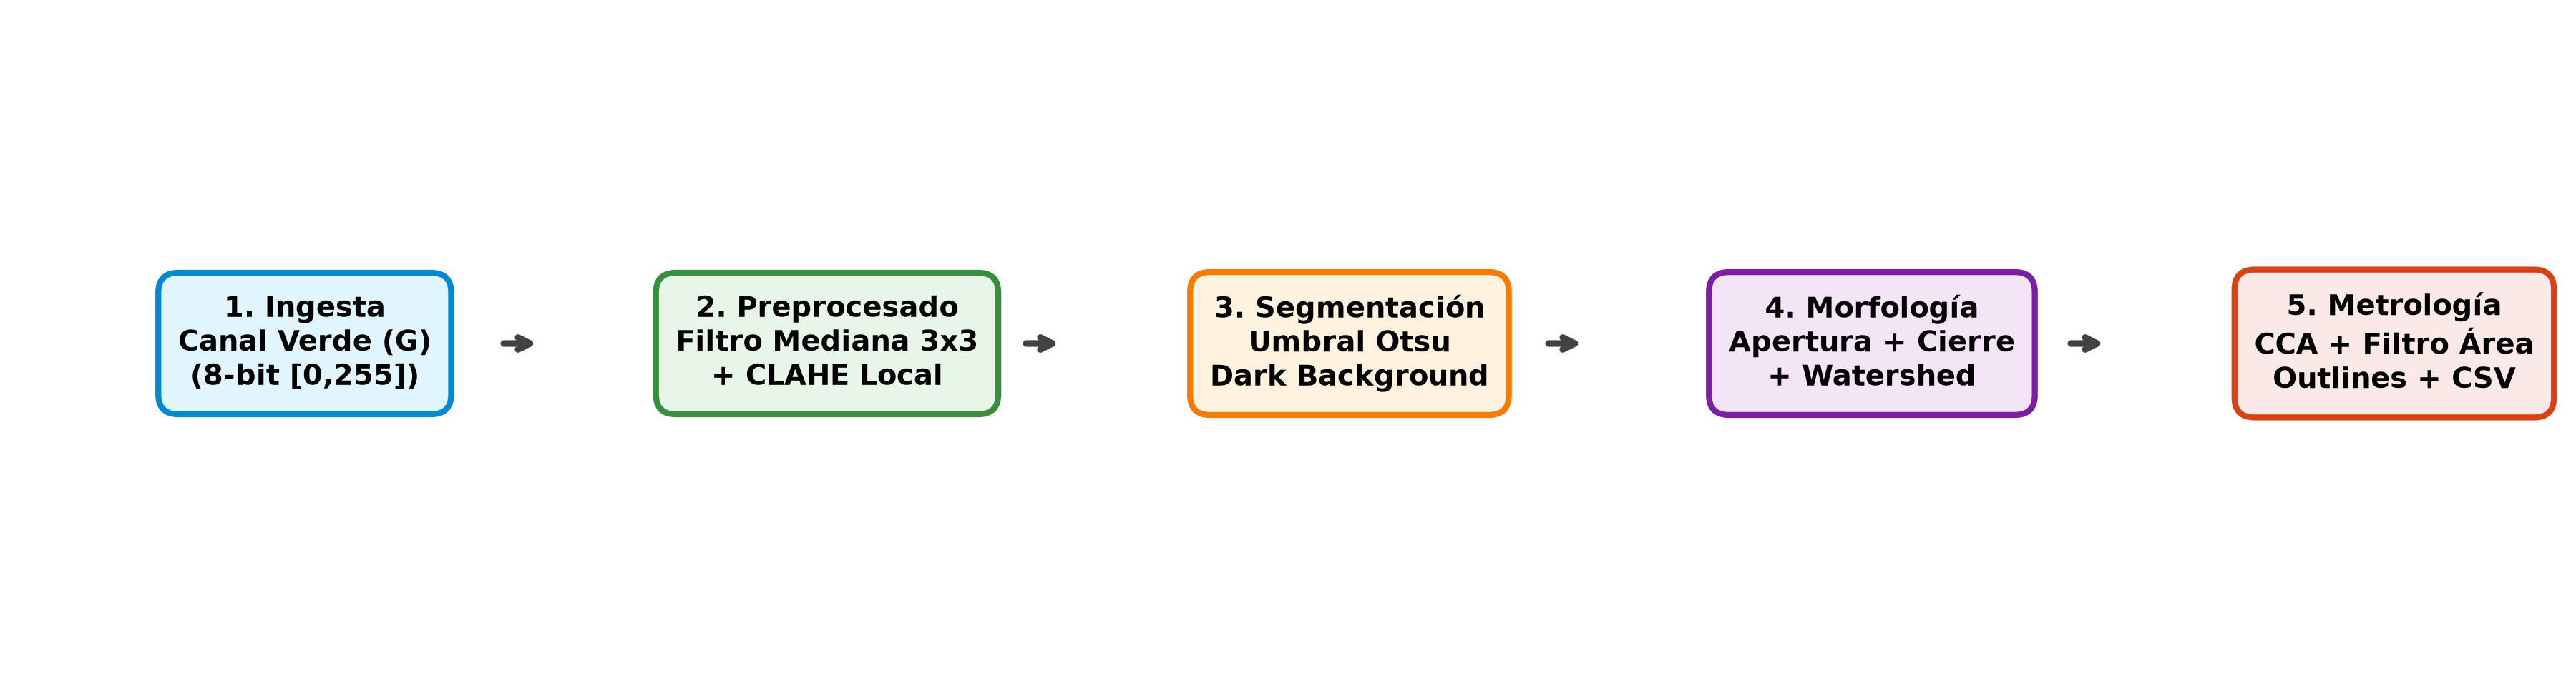
\includegraphics[width=0.95\textwidth]{figuras/fig2_flujograma_pipeline.png}
    \caption{Secuencia de bloques de las 5 etapas aplicadas en el pipeline de procesamiento.}
    \label{fig:flujo}
\end{figure}

\begin{table}[H]
\centering
\footnotesize
\begin{tabular*}{\textwidth}{@{\extracolsep{\fill}}llll@{}}
\toprule
\textbf{Etapa} & \textbf{Operación} & \textbf{Ruta en Fiji / ImageJ} & \textbf{Parámetros Exactos} \\ \midrule
1. Ingesta & Canal Verde 8-bit & \texttt{Image > Color > Split Channels} & Selección canal G ($[0, 255]$) \\
           & Histograma & \texttt{Analyze > Histogram} & 256 bins (Región FOV) \\
2. Preproceso & Filtro Espacial & \texttt{Process > Filters > Median...} & Radio $= 1.5\text{ px}$ (Kernel $3\times 3$) \\
              & Realce Local & \texttt{Process > Enhance Local Contrast} & Block=63, Bins=256, Slope=2.5 \\
              & Sustracción Fondo & \texttt{Process > Subtract Background} & Rolling ball $= 30\text{ px}$ \\
3. Segmentación & Umbralización & \texttt{Image > Adjust > Threshold} & \textbf{Otsu} ($T = 42$), \textit{Dark bg} \\
4. Morfología & Apertura Binaria & \texttt{Process > Binary > Open} & Disco $r=1\text{ px}$ ($3\times 3$) \\
              & Cierre y Relleno & \texttt{Process > Binary > Close / Fill Holes} & Sella huecos internos ($r=2$) \\
              & División de Aguas & \texttt{Process > Binary > Watershed} & Mapa distancia euclídea \\
5. Metrología & Set Measurements & \texttt{Analyze > Set Measurements} & Area, Centroid, Perim., Circ. \\
              & Conteo y Medición & \texttt{Analyze > Analyze Particles} & Size: \texttt{20-Inf}, \textit{Exclude edges} \\ \bottomrule
\end{tabular*}
\caption{Detalle de menús y parámetros configurados en cada etapa.}
\end{table}

% ==========================================
% 4. JUSTIFICACIÓN TEÓRICA Y ANALÍTICA
% ==========================================
\section{Justificación Teórica y Analítica}

\textbf{1. Filtro de Mediana ($3\times 3$) vs. Filtro Gaussiano o de Media:}
Probamos inicialmente un filtro Gaussiano, pero al ser un filtro lineal de promedio ponderado, difumina los bordes de las venas más finitas (capilares de 1 a 3 píxeles de grosor), haciendo que se pierdan al binarizar. En cambio, el \textbf{Filtro de Mediana} con ventana de $3\times 3$ (radio $1.5\text{ px}$) es un filtro no lineal de orden que suaviza la granulosidad del ruido térmico pero preserva los bordes nítidos (\textit{edge-preserving}). Elegimos un kernel pequeño de $3\times 3$ porque una ventana mayor ($5\times 5$ o $7\times 7$) borraría las ramificaciones vasculares más delgadas.

\begin{figure}[H]
    \centering
    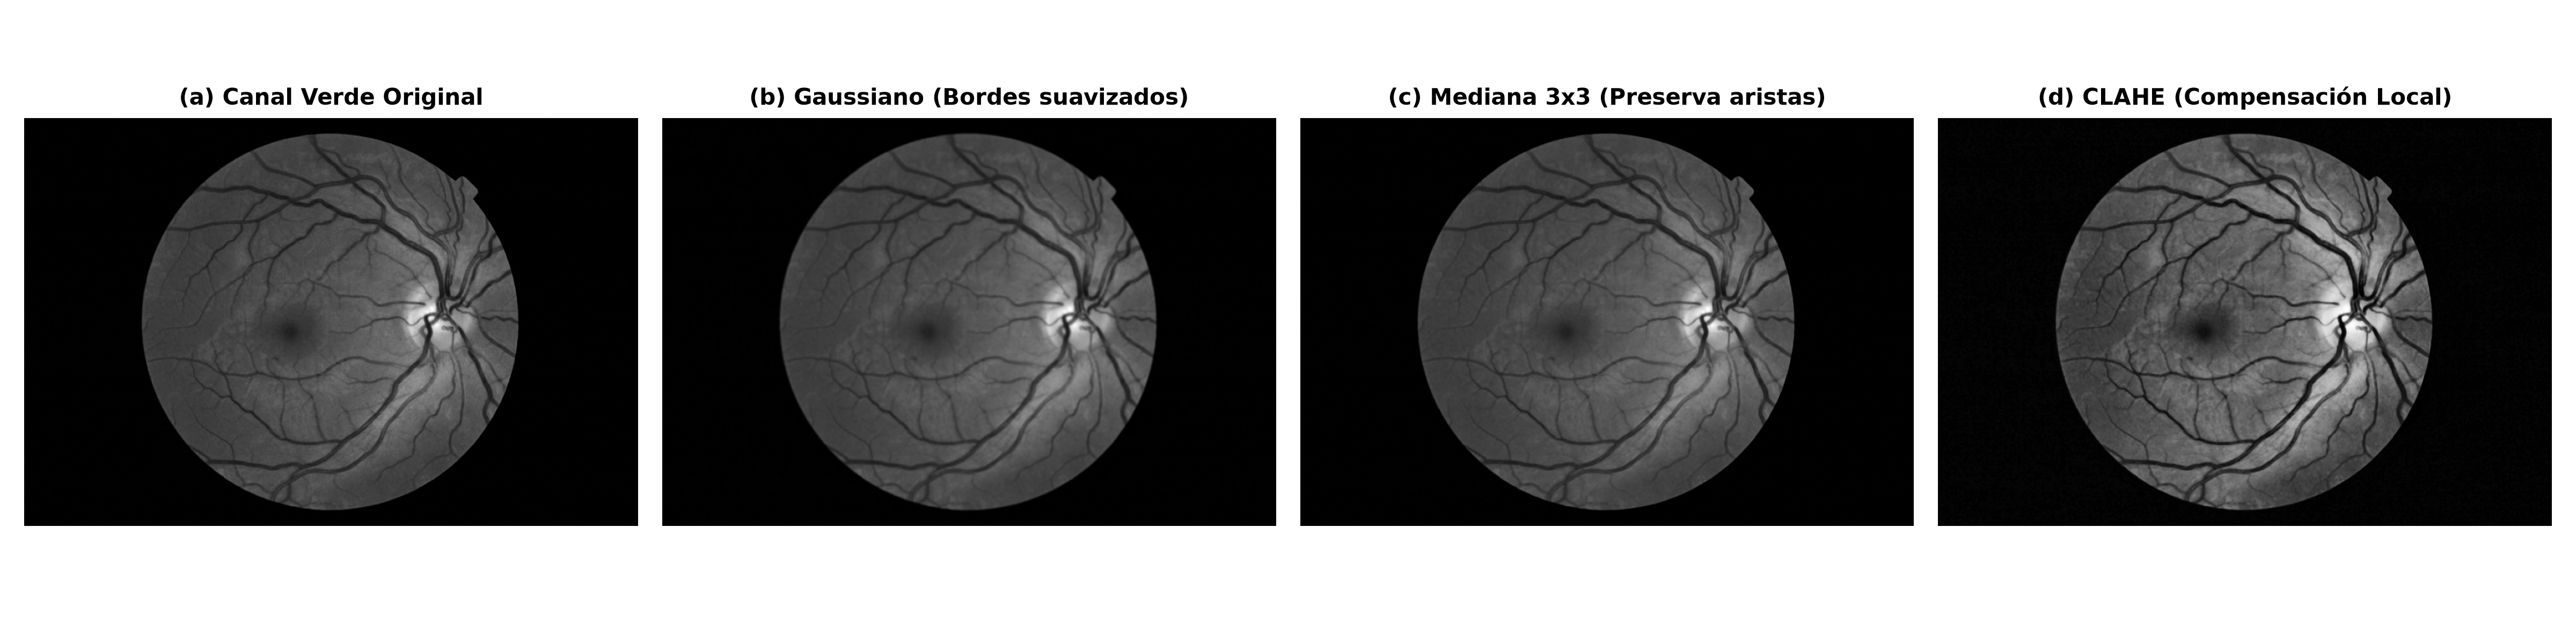
\includegraphics[width=0.95\textwidth]{figuras/fig4_comparativa_filtros_clahe.png}
    \caption{Comparación visual: el filtro de Mediana conserva los vasos finos y CLAHE levanta el contraste en zonas oscuras.}
    \label{fig:filtros}
\end{figure}

\textbf{2. Ecualización Adaptativa CLAHE vs. Ecualización Global:}
Una ecualización global de histograma estira el contraste tomando toda la imagen por igual; como el centro de la retina es brillante y los bordes son oscuros, la ecualización global quema la zona del nervio óptico y mete mucho ruido en la periferia. Por eso aplicamos \textbf{CLAHE}, que trabaja por bloques locales y limita la pendiente máxima (\textit{clip limit} de $2.5$). Así logramos resaltar las venas en las zonas oscuras sin saturar el centro, acompañado de una sustracción de fondo (\textit{Rolling Ball} de $30\text{ px}$) para emparejar la iluminación general.

\textbf{3. Umbral de Otsu vs. Umbral Manual y Polaridad:}
El algoritmo de \textbf{Otsu} busca automáticamente el umbral que maximiza la varianza entre dos clases (vasos y fondo), dando un valor exacto de $T = 42$. Al compararlo con un ajuste manual empírico, vimos que bajar el umbral manualmente a $T \approx 30$ permite recuperar algunos microcapilares más, pero mete muchísimo ruido de fondo que ensucia las mediciones; subirlo a $T > 55$ corta las arterias principales en pedazos. Por lo tanto, el umbral de Otsu ($T = 42$) resultó el punto de equilibrio más objetivo y reproducible. Se activó \textit{Dark background} sobre el mapa de vasos realzado para que los vasos queden blancos ($255$) y el fondo negro ($0$).

\textbf{4. Operaciones Morfológicas y Watershed:}
\begin{itemize}
    \item \textbf{Apertura (\textit{Open}):} Aplica erosión seguida de dilatación. Nos sirvió para borrar pequeños puntitos blancos aislados y espículas en los bordes que quedaron tras binarizar.
    \item \textbf{Cierre (\textit{Close}) y Relleno (\textit{Fill Holes}):} Las arterias suelen tener un brillo central que al binarizar deja huecos alargados adentro del vaso. El cierre y relleno sellan esos poros internos para que el vaso sea compacto.
    \item \textbf{Watershed:} En una red vascular todas las ramas se tocan o cruzan. Al aplicar \textit{Watershed}, Fiji calcula el mapa de distancia al borde y corta los estrechamientos y cruces, separando el árbol vascular en segmentos medibles por separado sin caer en una sobre-segmentación excesiva.
\end{itemize}

% ==========================================
% 5. MEMORIA GRÁFICA DE TRANSFORMACIÓN
% ==========================================
\section{Memoria Gráfica de Transformación}

En la siguiente galería se muestra paso a paso la evolución de la imagen a lo largo de las 5 etapas del pipeline:

\begin{figure}[H]
    \centering
    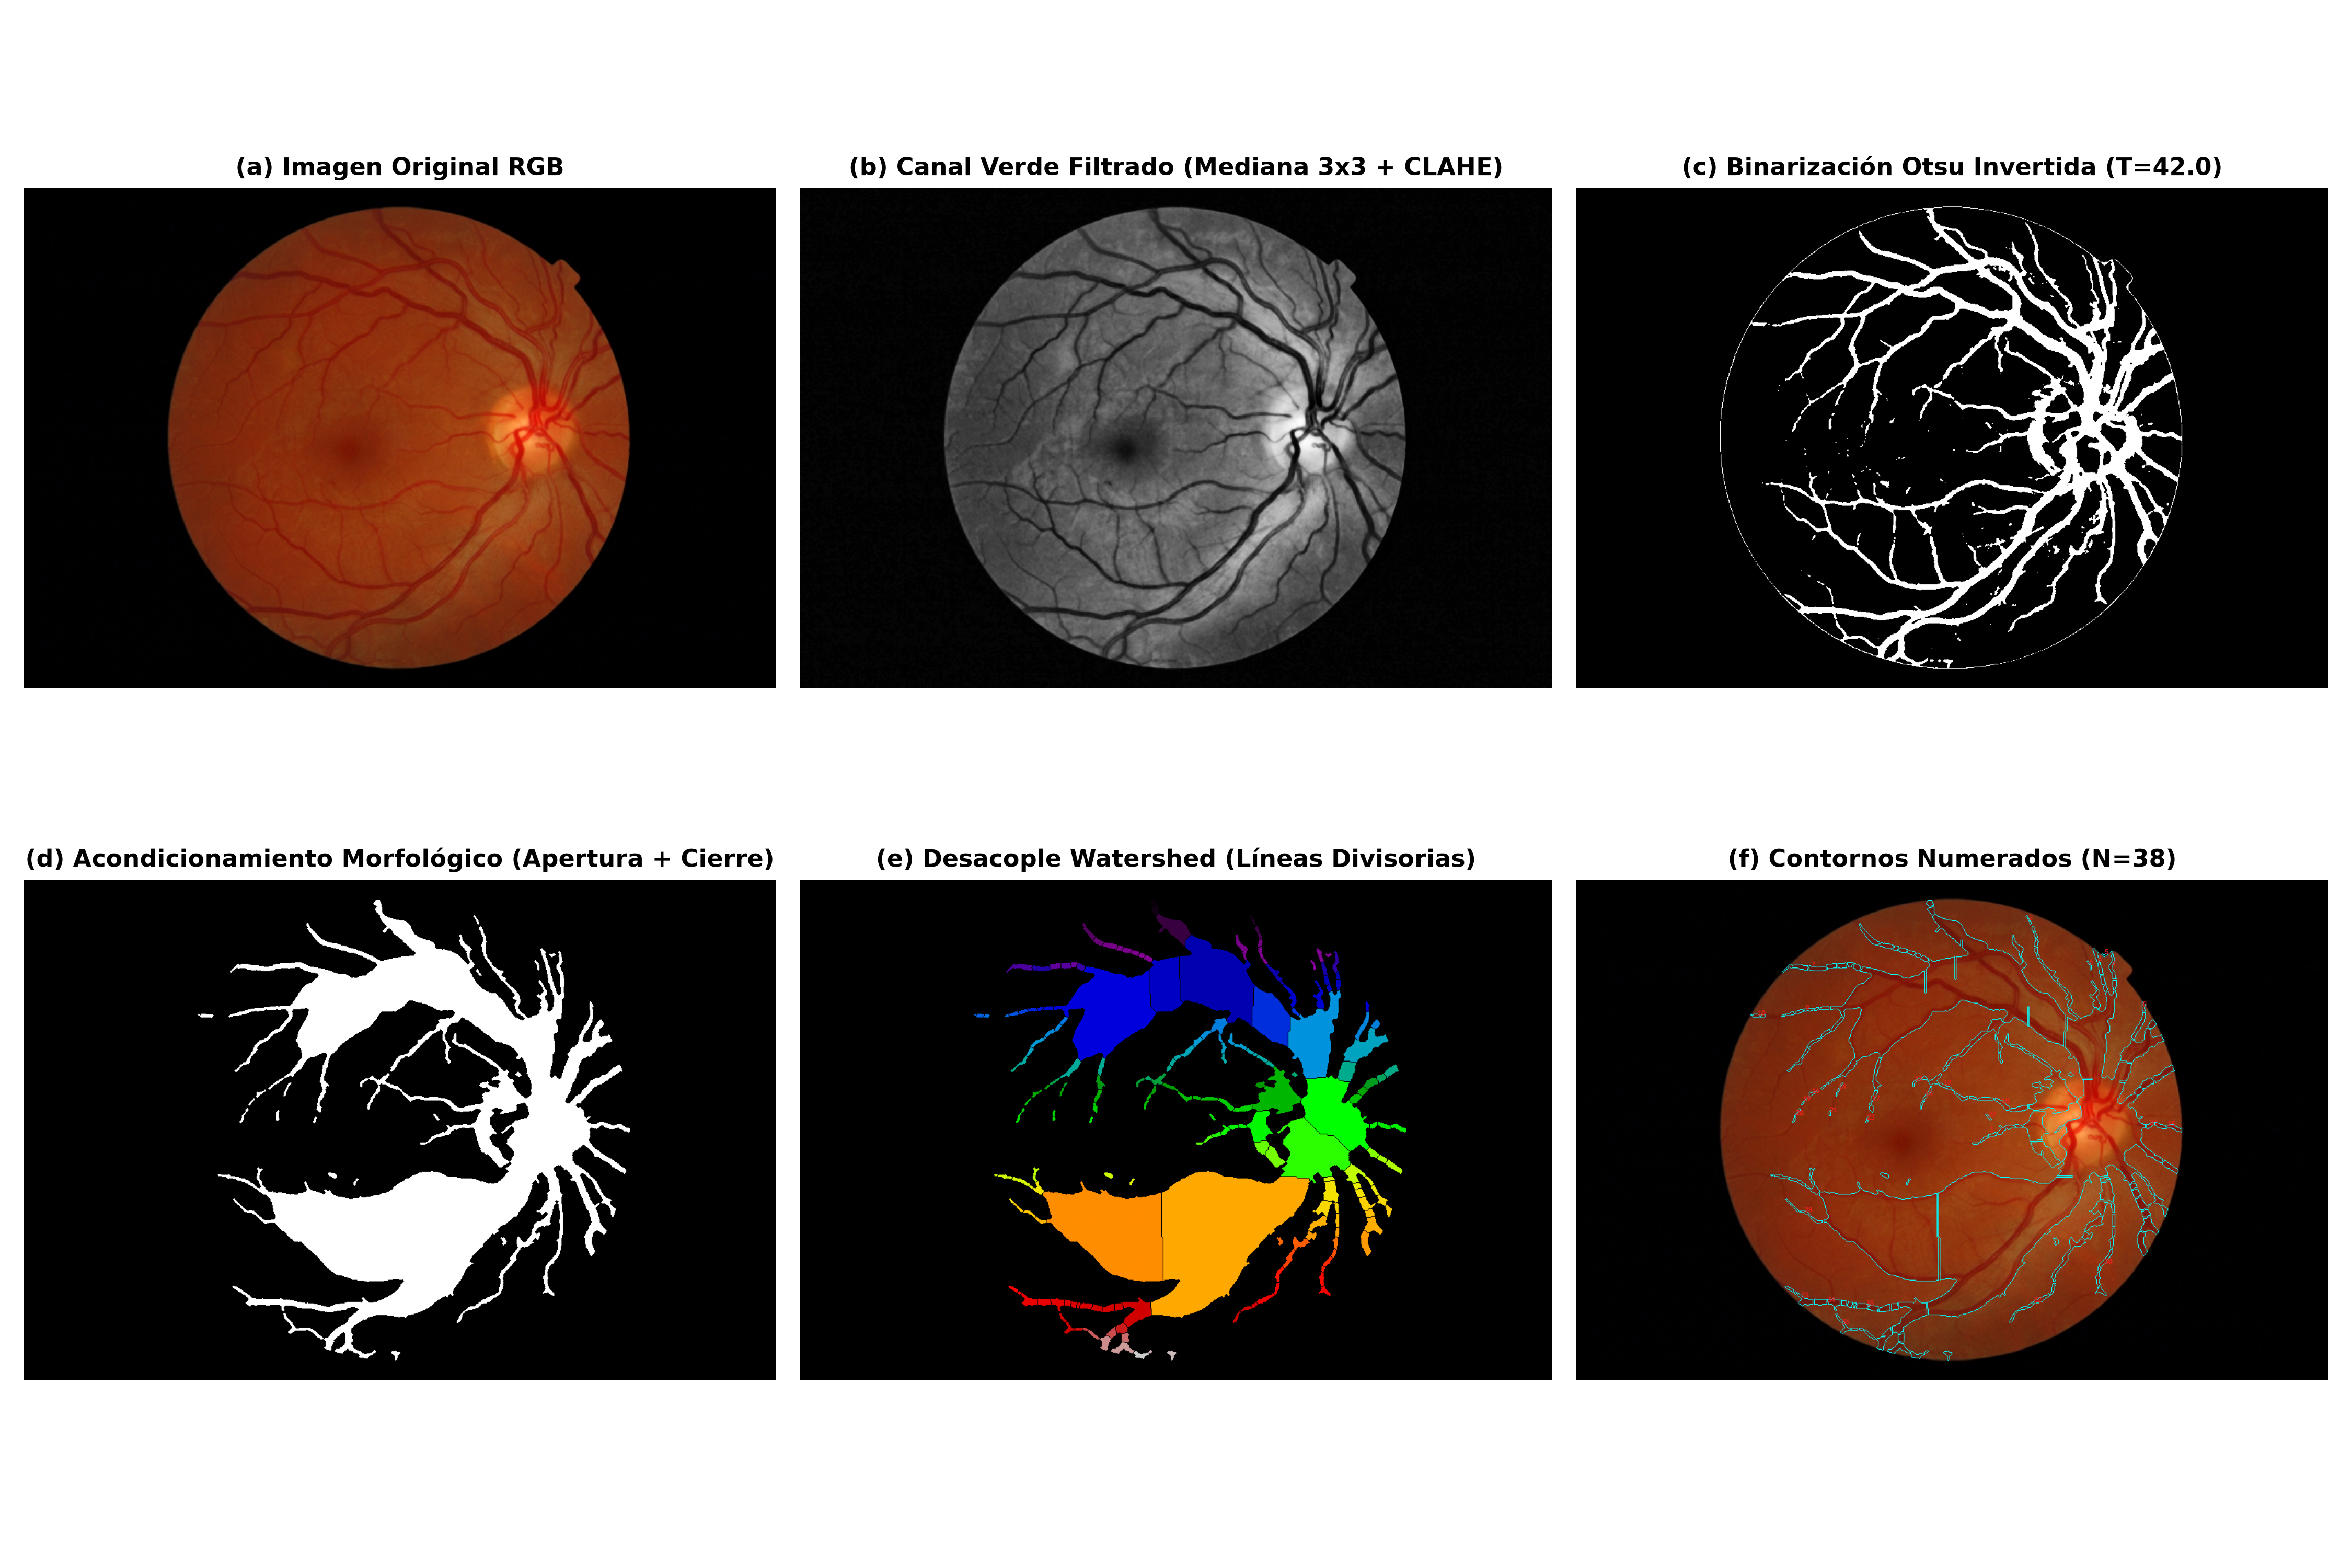
\includegraphics[width=0.96\textwidth]{figuras/fig3_memoria_grafica_etapas.png}
    \caption{Memoria gráfica comparativa de las transformaciones: (a) Imagen Original; (b) Filtrada con Mediana y realzada con CLAHE; (c) Binarizada con Otsu ($T=42$); (d) Morfología binaria (Apertura y Cierre); (e) Separación de ramas con Watershed; (f) Mapa final de contornos numerados.}
    \label{fig:memoria}
\end{figure}

% ==========================================
% 6. CUADRO ESTADÍSTICO Y METROLOGÍA
% ==========================================
\section{Cuadro Estadístico y Metrología}

Para la Etapa 5 configuramos \texttt{Analyze Particles} filtrando el ruido residual menor a $20\text{ px}^2$ y marcando \textit{Exclude on edges} para descartar los segmentos que tocan los bordes de corte. Los resultados exportados en el archivo CSV se resumen en la siguiente tabla:

\begin{table}[H]
\centering
\begin{tabular}{@{}lc@{}}
\toprule
\textbf{Métrica / Descriptor Metrológico} & \textbf{Valor Obtenido} \\ \midrule
Recuento total de objetos válidos ($N$) & \textbf{38 segmentos vasculares} \\
Área útil del fondo de ojo (FOV de referencia) & $311\,605\text{ px}^2$ \\
Área total ocupada por vasos sanguíneos & $101\,901.00\text{ px}^2$ \\
Área media por objeto ($\mu_A$) & $2\,681.61\text{ px}^2$ (Mediana: $78.00\text{ px}^2$) \\
Área mínima registrada & $22.00\text{ px}^2$ \\
Área máxima registrada (tronco vascular principal) & $96\,280.00\text{ px}^2$ \\
Desviación estándar del área ($\sigma_A$) & $15\,594.71\text{ px}^2$ \\
Circularidad promedio ($C = \frac{4\pi \cdot \text{Área}}{\text{Perímetro}^2}$) & \textbf{0.4399} (Mediana: \textbf{0.3287}) \\
\textbf{Porcentaje de ocupación superficial vascular} & \textbf{32.70\%} \\ \bottomrule
\end{tabular}
\caption{Resumen estadístico de las mediciones obtenidas sobre la retina.}
\end{table}

\textbf{Análisis de los resultados numéricos:}
Llama la atención que la \textbf{circularidad promedio sea baja ($0.4399$ y mediana de $0.3287$)}. Esto tiene total sentido físico y anatómico: a diferencia de monedas o células redondas (donde $C$ ronda $0.85$ a $1.0$), los vasos sanguíneos son estructuras tubulares largas, finas y ramificadas, lo que hace que tengan muchísimo perímetro en relación a su área. Asimismo, la gran diferencia entre el área media ($2\,681\text{ px}^2$) y la mediana ($78\text{ px}^2$) se debe a que el árbol vascular principal mantiene una estructura grande conectada mientras que las ramificaciones periféricas desacopladas por Watershed son segmentos más cortos.

% ==========================================
% 7. AUDITORÍA DE ERRORES Y CONCLUSIONES
% ==========================================
\section{Auditoría de Errores y Conclusiones}

\textbf{Auditoría crítica de errores observados:}
\begin{enumerate}
    \item \textbf{Casos de Sub-segmentación (pérdida de capilares finos):} En la zona izquierda e inferior de la retina (donde la iluminación original era más débil), los capilares más finitos tienen un contraste muy bajo. Al aplicar un único umbral global de Otsu ($T=42$) y luego una apertura morfológica, varios de estos microvasos delgados quedan desconectados o por debajo del corte de $20\text{ px}^2$.
    \item \textbf{Casos de Sobre-segmentación y artefactos:} En la zona brillante del disco óptico (derecha) y en algunas bifurcaciones anchas, el algoritmo de \textit{Watershed} (pensado originalmente para objetos convexos o circulares como células) genera cortes transversales artificiales sobre venas que en realidad son un mismo conducto continuo.
\end{enumerate}

\textbf{Propuestas de optimización:}
\begin{itemize}
    \item \textbf{Umbralización Local Adaptativa (Phansalkar o Bernsen):} En lugar de usar Otsu global, usar \texttt{Image > Adjust > Auto Local Threshold} en Fiji permitiría adaptarse mejor a los microvasos en regiones oscuras sin engrosar las venas del centro.
    \item \textbf{Filtros Tubulares (Frangi Vesselness / Tubeness):} Fiji incluye el plugin \texttt{Plugins > Analyze > Tubeness}, que detecta específicamente formas cilíndricas o lineales antes de binarizar, evitando que se corten los capilares finos y reemplazando el uso de Watershed por un análisis de esqueleto (\texttt{Skeletonize}).
\end{itemize}

\textbf{Conclusión:}
El pipeline desarrollado en 5 etapas permitió acondicionar con éxito una imagen médica compleja con iluminación despareja y bajo contraste local. La combinación del canal verde, el filtro de Mediana ($3\times 3$) y el realce CLAHE fue clave para que la segmentación de Otsu y la morfología binaria lograran aislar la red vascular, determinando una ocupación superficial del $32.70\%$ y verificando cuantitativamente su geometría alargada mediante el descriptor de circularidad.

\end{document}
